\documentclass[11pt,a4paper]{article}
\usepackage[UTF8]{ctex}
\usepackage[margin=2.3cm]{geometry}
\usepackage{graphicx}
\usepackage{booktabs}
\usepackage{longtable}
\usepackage{array}
\usepackage{amsmath}
\usepackage{float}
\usepackage{caption}
\usepackage{xcolor}
\usepackage{titlesec}
\usepackage[hidelinks]{hyperref}

\graphicspath{{assets/}}

\titleformat{\section}{\large\bfseries}{\thesection}{0.8em}{}
\titleformat{\subsection}{\normalsize\bfseries}{\thesubsection}{0.8em}{}
\titlespacing*{\section}{0pt}{1.1ex}{0.6ex}
\titlespacing*{\subsection}{0pt}{0.9ex}{0.4ex}

\captionsetup{font=small,labelfont=bf}
\setlength{\parskip}{0.3em}

\begin{document}

\begin{center}
{\LARGE\bfseries Week 8 实验报告}\\[0.3em]
{\large 工具功能完善与项目交付——可部署定价工具、最终报告与演示}\\[0.2em]
{\small Final Project Delivery --- Deployable Pricing Tool, Final Report \& Demo}\\[0.4em]
{\small 2026 年 8 月 26 日}
\end{center}

\section{项目概述与目标}

选择权期权（Chooser Option）赋予持有人在未来选择日 $t_1$ 决定该期权是欧式看涨还是欧式看跌的权利，并设定统一行权价 $K$ 与最终到期 $T_2$。本项目用 8 周时间，从真实市场数据出发，复现基于 BSM 的选择权定价模型，并以机器学习（ML）方法优化其"恒定波动率"局限，最终交付一个数据驱动、可部署的双轨定价工具。

第 8 周为项目收尾，关键任务与交付物为：

\begin{itemize}
  \item \textbf{工具功能完善}：实现 BSM + 最优 ML 模型的最终双轨定价；添加误差范围显示；完善可视化仪表板（价格趋势、敏感性图表、性能指标）。
  \item \textbf{最终报告}：将全部 8 周发现整合为 10--15 页报告。
  \item \textbf{演示准备}：录制工具演示视频、制作最终演示文稿。
\end{itemize}

对应交付物：可部署定价工具（含 README 的 GitHub 仓库）、最终项目报告（PDF）、工具演示视频脚本（5--10 分钟）、最终演示文稿。

\section{总体架构与实验流程}

项目采用"学术模型（BSM）$\to$ 机器学习增强 $\to$ 工具化部署"的三阶段推进。第 1--2 周完成数据采集与特征工程；第 3--4 周复现 BSM 模型并建立性能基线；第 5--6 周建立双轨 ML 架构并完成训练、调优与比较；第 7 周完成高级敏感性与工具原型；第 8 周（本报告）完成工具功能、最终报告与演示。

\begin{center}
\begin{tabular}{@{}l@{\quad}p{0.72\linewidth}@{}}
\toprule
\textbf{阶段} & \textbf{内容} \\
\midrule
第 1--2 周 & 数据采集（JPM 日线、VIX、3M 国债，2018--2024）与 16+ 维特征工程、自动化预处理流水线 \\
第 3--4 周 & BSM（Rubinstein）选择权定价模型复现与基线评估（$K=\$150$、$T_2=1$ 年） \\
第 5 周 & 双轨 ML 架构：方法一（ML 波动率预测 $+$ BSM 定价）、方法二（端到端监督定价） \\
第 6 周 & 超参优化（purged 时序 CV）、最终模型训练与测试集比较、SHAP/LIME 可解释性 \\
第 7 周 & SHAP$\times$Vega 敏感性分解、极端场景测试、Streamlit 原型、实时数据集成 \\
\textbf{第 8 周} & \textbf{工具功能完善（双轨定价、误差条、完整仪表板）、最终报告、演示文稿} \\
\bottomrule
\end{tabular}
\end{center}

\section{数据与特征工程（第 1--2 周）}

\subsection{数据采集}

以 Yahoo Finance / Alpha Vantage / FRED 为数据源，采集 2018-01--2024-12 的 JPM 日线（OHLCV）、VIX 指数与 3M 国债收益率。经时间对齐与清洗（缺失值插值、IQR 异常值剔除）后得到结构化特征数据集 \textbf{1755 行、20 列}，覆盖 2018-01-09 至 2024-12-30。

\subsection{特征工程}

在基础特征（5/21/63 日滚动波动率、日收益率、股息增长率、区间振幅、成交量变化）之上，加入面向市场情绪与波动率联动的"新特征"：

\begin{itemize}
  \item \textbf{sentiment\_score}：由 VIX 在 252 日区间内的位置构造（0--1），刻画市场恐慌/情绪状态；
  \item \textbf{vix\_ratio}、\textbf{vix\_change\_1d}、\textbf{vix\_jpm\_corr\_21d}、\textbf{vix\_jpm\_cross\_1d}：VIX 相对已实现波动率溢价、VIX 动量与 JPM--VIX 联动；
  \item \textbf{rate\_change\_1d\_bps}、\textbf{rate\_momentum\_5d\_bps}：利率变动与动量。
\end{itemize}

全部特征经后视窗口构造以避免前瞻偏差，并配套 GitHub Actions 调度的自动化预处理流水线。

\section{BSM 选择权定价模型复现与基线（第 3--4 周）}

\subsection{模型公式}

采用 Rubinstein (1991) 简单选择权定价公式，参数对齐论文：$K=\$150$、$T_2=1$ 年、选择日 $t_1=0.5$ 年：

\begin{equation}
  P_{\mathrm{chooser}} = C(S,K,T_2) + P(S,Ke^{-q(T_2-t_1)},t_1)
\end{equation}

其中 $C/P$ 为标准欧式看涨/看跌（BS 公式），$q$ 为股息率。模型代码与论文参数配置经 Jupyter Notebook 复现并通过与论文结果的初始对比验证。

\subsection{基线评估（第 4 周）}

以 2026-07-27 实盘快照（595 张合约）与合成测试集建立 BSM(vol\_21d) 基线：
\begin{itemize}
  \item 实盘基线：MAE $\$1.44$、ATM IV 溢价 $4.9\%$、OTM 看跌定价偏差 $-65.7\%$；
  \item 合成测试集（2024，208 日）Chooser 定价 MAE $\$1.52$。
\end{itemize}

该基线为后续所有 ML 模型提供了统一比较口径。

\section{机器学习双轨架构（第 5 周）}

\begin{itemize}
  \item \textbf{方法一（波动率预测 $+$ BSM 定价）}：LSTM / RandomForest / GBDT / XGBoost 预测 BSM 唯一不确定的输入——波动率 $\sigma$——再经 BSM 引擎定价；另设 VIX-proxy 模型（预测 VIX$_{t+1}$，以 VIX/100 作为 $\sigma$）以逼近"以市场隐含波动率为目标"的设计意图。
  \item \textbf{方法二（端到端监督定价）}：线性回归 / GBDT / MLP 直接预测期权价格（合约网格特征 $+$ 市场特征）。
  \item \textbf{反前瞻保障}：时序 70/15/15 分割、特征后视、目标错位、Scaler 训练集拟合等六重防护。
\end{itemize}

\section{模型训练、调优与比较（第 6 周）}

\subsection{超参优化}

以扩张窗口 $+$ 21 日 embargo 的 purged 时序交叉验证 + 随机搜索，系统性加大正则（浅树、小学习率、高叶约束、L1/L2）。XGBoost 最优 CV-MAE 收敛至 $6.99\%$，逼近 persistence 基线（$7.32\%$）；GBDT/GBDT-anchored 较默认超参改善 $-20\%$ 级。

\begin{figure}[H]
  \centering
  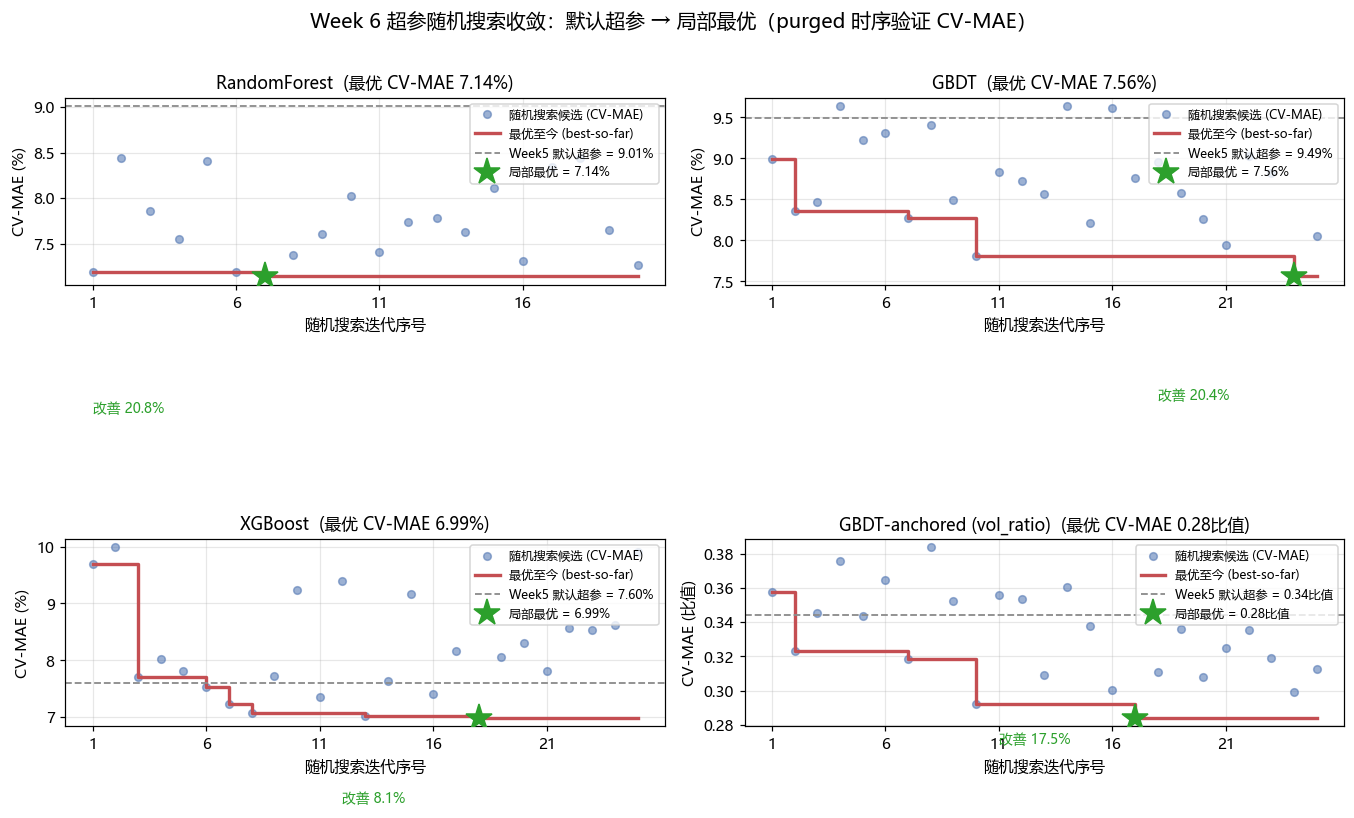
\includegraphics[width=0.82\linewidth]{fig_w6_hp_convergence.png}
  \caption{随机搜索收敛路径：候选点 CV-MAE（蓝点）、最优至今曲线（红线）与 Week 5 默认超参基线（灰虚线）。}
\end{figure}

\subsection{测试集评估（2024，208 日）}

\subsubsection{方法一：波动率预测}

\begin{table}[H]
  \centering
  \caption{波动率预测误差（测试集 208 日）}
  \begin{tabular}{lcccc}
    \toprule
    模型 & MAE (\%) & RMSE (\%) & R$^2$ \\
    \midrule
    \textbf{GBDT-anchored (vol\_ratio)} & \textbf{7.16} & 9.29 & $-0.11$ \\
    BSM($\sigma_{21d}$) persistence（基线） & 7.32 & 8.95 & $-0.03$ \\
    XGB-VIX proxy (IV) & 7.46 & 9.24 & $-0.10$ \\
    GBDT & 8.36 & 11.27 & $-0.63$ \\
    RandomForest & 8.36 & 11.25 & $-0.63$ \\
    XGBoost & 8.42 & 12.06 & $-0.87$ \\
    LSTM & 10.92 & 15.57 & $-2.12$ \\
    \bottomrule
  \end{tabular}
\end{table}

调优后的 \textbf{GBDT-anchored 以 MAE=7.16\% 首次超越 persistence 基线（7.32\%）}，实现了波动率预测越过强基线的里程碑。

\subsubsection{方法一：Chooser 定价（BSM 混合引擎）}

\begin{table}[H]
  \centering
  \caption{Chooser 期权定价误差（测试集，vs 前向波动率公平价）}
  \begin{tabular}{lcccc}
    \toprule
    模型 & MAE (\$) & RMSE (\$) & R$^2$ & bias \\
    \midrule
    \textbf{XGB-VIX proxy (IV)} & \textbf{1.17} & 1.69 & 0.982 & $-0.58$ \\
    BSM($\sigma_{21d}$) 基线 & 1.52 & 2.17 & 0.970 & $+0.07$ \\
    GBDT-anchored & 1.55 & 2.71 & 0.953 & $+0.21$ \\
    RandomForest & 1.60 & 2.92 & 0.945 & $+0.37$ \\
    XGBoost & 1.71 & 3.32 & 0.929 & $+0.91$ \\
    GBDT & 1.72 & 2.75 & 0.951 & $+0.88$ \\
    LSTM & 2.63 & 4.17 & 0.888 & $+1.32$ \\
    \bottomrule
  \end{tabular}
\end{table}

\textbf{Week 6 最重要的定价结果}：VIX-proxy 以 MAE=\$1.17 大幅超越 BSM 基线（\$1.52），改善 \textbf{23\%}。市场隐含波动率（VIX 代理）直接编码了市场对未来波动率的预期（IV premium），经 BSM 引擎定价后与公平价偏差最小。图 \ref{fig:w6_chooser} 为测试集误差的可视化。

\begin{figure}[H]
  \centering
  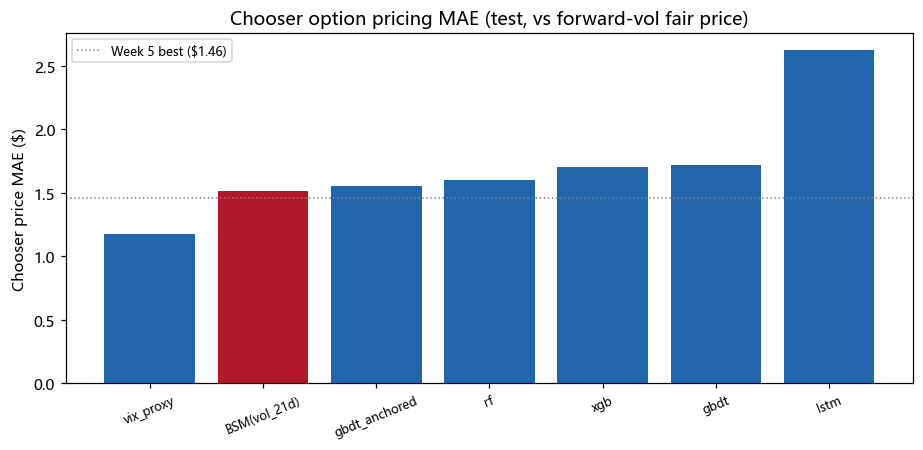
\includegraphics[width=0.85\linewidth]{fig_w6_chooser_price_mae.png}
  \caption{方法一：Chooser 定价测试集误差（MAE，2024）。VIX-proxy 显著优于 BSM 基线。}
  \label{fig:w6_chooser}
\end{figure}

\subsubsection{方法二：端到端定价}

\begin{table}[H]
  \centering
  \caption{端到端期权定价误差（合约网格，2024）}
  \begin{tabular}{lcccc}
    \toprule
    模型 & MAE (\$) & RMSE (\$) & R$^2$ \\
    \midrule
    BSM($\sigma_{21d}$) 静态基准 & \textbf{1.77} & 2.24 & 0.930 \\
    GBDT（调优后） & 3.69 & 4.86 & 0.670 \\
    MLP-NN（调优后） & 4.61 & 5.92 & 0.510 \\
    \bottomrule
  \end{tabular}
\end{table}

方法二调优后改善但无法超越静态 BSM 基准——将 ML 能力集中于 BSM 唯一不确定的输入（波动率）优于让模型独立重建定价函数。该结论确定了双轨定价中"方法一为首选"的最终架构。

\subsection{实盘指标验证}

在 2026-07-27 快照（595 张合约）上，调优后的 \textbf{XGBoost} 同时满足全部三项 Week 6 目标：

\begin{table}[H]
  \centering
  \caption{实盘指标：Week 4 基线 / Week 6 最优（XGB）vs 目标}
  \begin{tabular}{lccccl}
    \toprule
    指标 & Week 4 基线 & Week 6 最优 (XGB) & 目标 & 达成 \\
    \midrule
    实盘 MAE (\$) & 1.44 & \textbf{0.79} & $<1.00$ & 达成 \\
    ATM IV 溢价 (\%) & 4.9 & \textbf{0.76} & $<2.0$ & 达成 \\
    OTM 看跌定价偏差 (\%) & $-65.7$ & \textbf{$-29.5$} & $>-30$ & 达成 \\
    \bottomrule
  \end{tabular}
\end{table}

\begin{figure}[H]
  \centering
  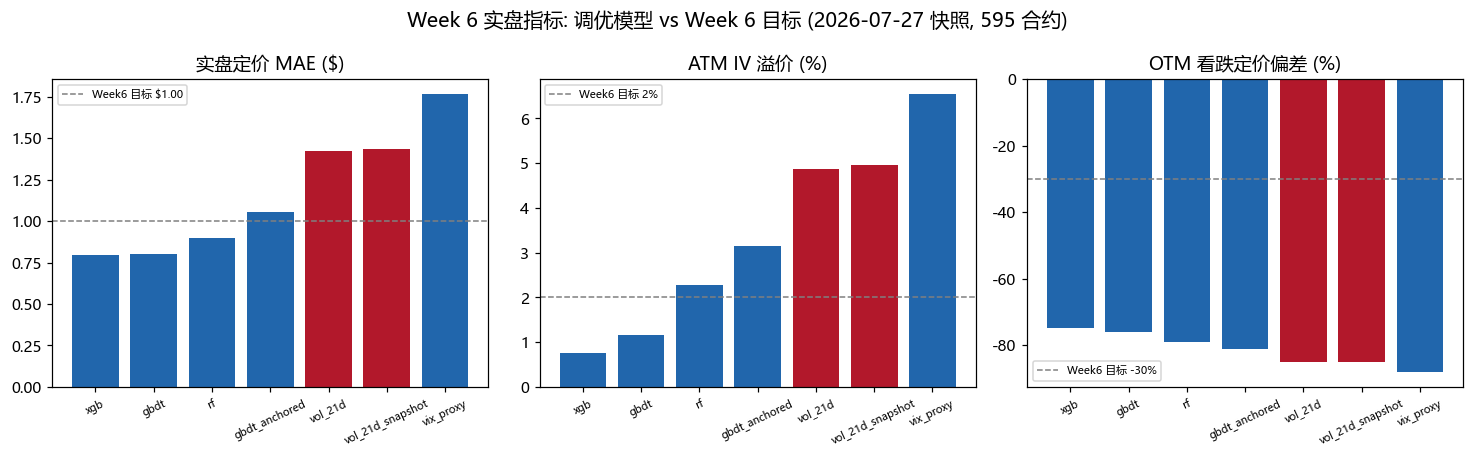
\includegraphics[width=0.85\linewidth]{fig_w6_live_metrics.png}
  \caption{Week 6 实盘指标：调优模型 vs Week 6 目标线。}
\end{figure}

\subsection{可解释性}

SHAP 分析显示 VIX-proxy 模型的重要性高度集中：sentiment\_score (1.69) 最显著，其后为 $\sigma_{63d}$ (0.51)、$\sigma_{21d}$ (0.36)、vix\_ratio (0.28)。以市场隐含波动率为目标时，波动率的\textbf{位置/状态特征}（sentiment、vix\_ratio）比原始水平特征更重要。图 \ref{fig:w6_shap} 为 mean-|SHAP| 全局重要性。

\begin{figure}[H]
  \centering
  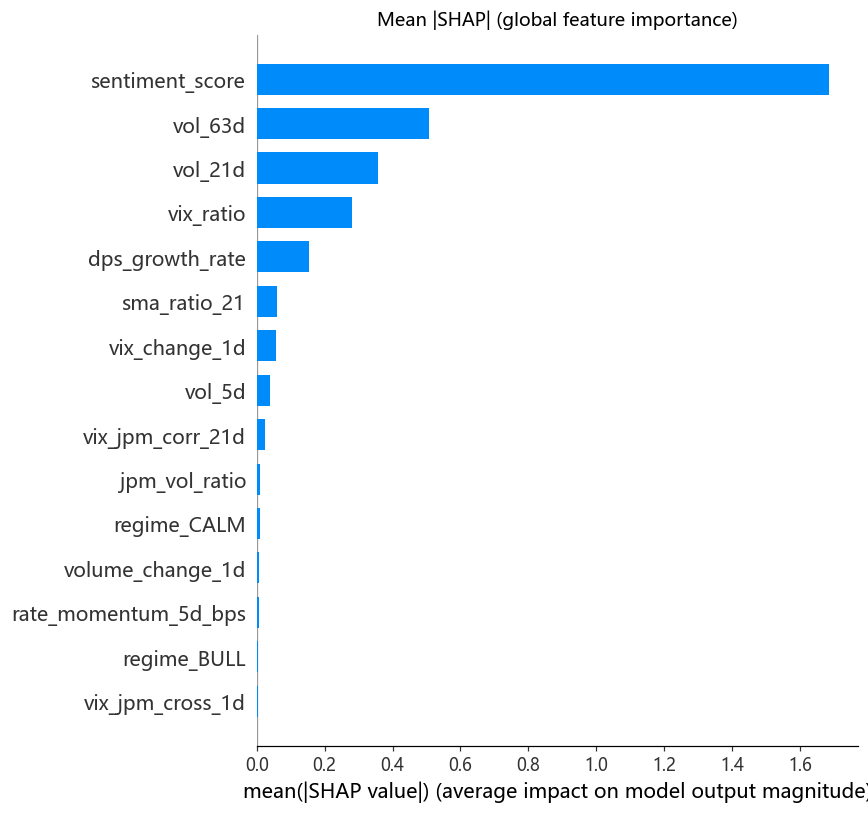
\includegraphics[width=0.75\linewidth]{fig_w6_shap_vix_proxy_bar.png}
  \caption{VIX-proxy 模型 SHAP 全局重要性。}
  \label{fig:w6_shap}
\end{figure}

\section{高级敏感性分析（第 7 周）}

\subsection{SHAP$\times$Vega 价格影响分解}

将"特征对 Chooser 价格的边际影响"沿 BSM 混合引擎拆成链条式——特征对波动率预测的 SHAP 贡献 $\times$ 价格对波动率的 Vega：

\begin{equation}
  \text{价格影响}_j = \mathrm{SHAP}_j(\hat\sigma) \cdot \frac{\partial\sigma}{\partial\text{target}} \cdot \frac{\partial P}{\partial\sigma}.
\end{equation}

\begin{figure}[H]
  \centering
  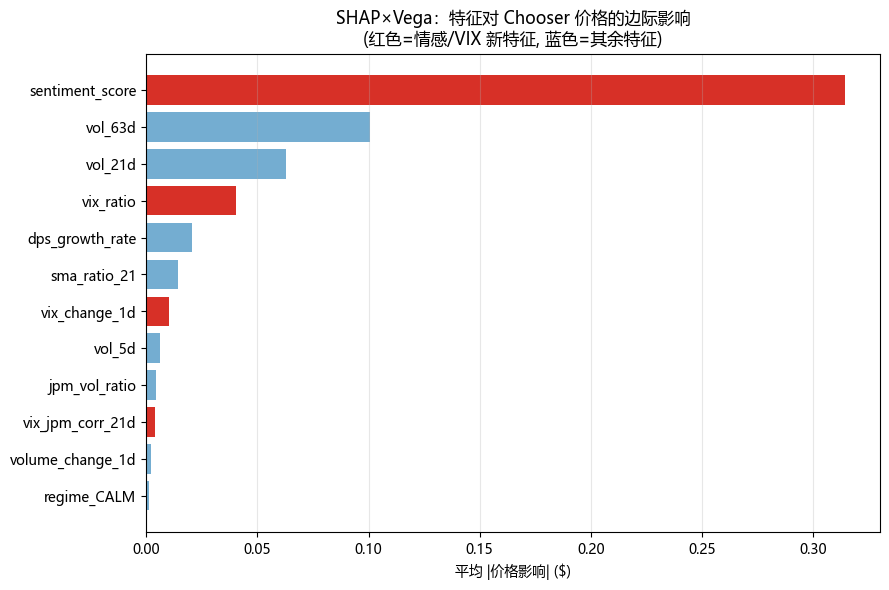
\includegraphics[width=0.78\linewidth]{fig_w7_shap_price_impact_vixproxy.png}
  \caption{VIX-proxy 模型 SHAP$\times$Vega 价格影响（红色=情感/VIX 新特征）。sentiment\_score 是最大单一价格驱动。}
\end{figure}

核心发现：\textbf{情感/VIX 新特征是最大单一价格驱动}。对 VIX-proxy 模型，sentiment\_score 的平均价格影响为 \$0.314（约为平均价格 \$57.9 的 0.54\%），是次高特征 vol\_63d（\$0.101）的 3 倍。

\subsection{极端场景测试}

\begin{figure}[H]
  \centering
  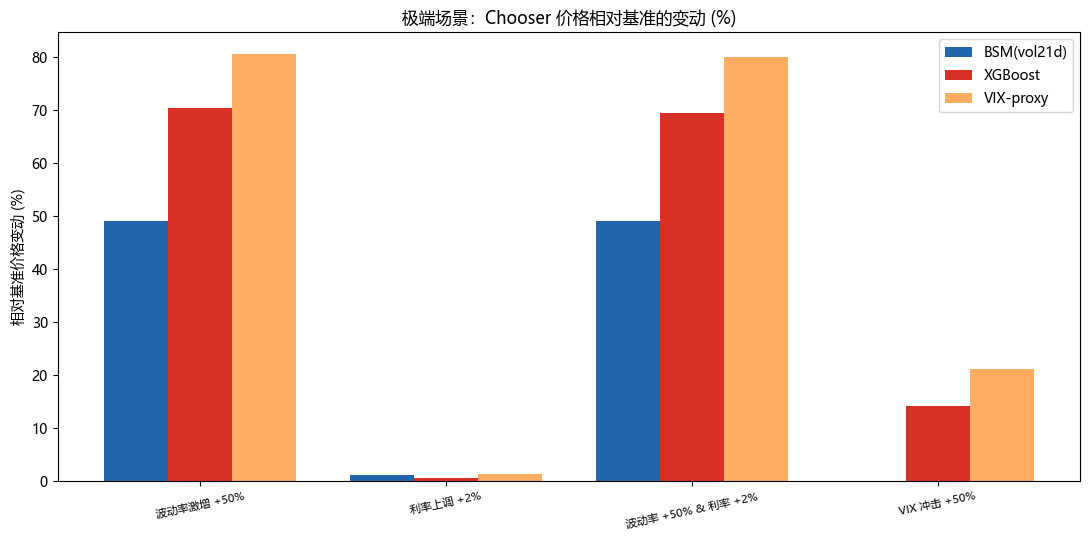
\includegraphics[width=0.88\linewidth]{fig_w7_scenarios_atm.png}
  \caption{ATM 基座（$S=K=150$）极端场景价格变动（\%）。ML 模型在波动率与 VIX 冲击下放大幅度明显大于 BSM。}
\end{figure}

ATM 基座下波动率 +50\% 使 BSM $+49.1\%$、XGB $+70.3\%$、VIX-proxy $+80.7\%$；VIX 冲击 +50\% 下 BSM 无反应（vol\_21d 不变），而 XGB $+14.2\%$、VIX-proxy $+21.1\%$——ML 模型通过特征重工程"感知"市场恐慌。而在实盘基座（$S=356.20$，深度实值 $S/K=2.37$）下 Chooser 波动率不敏感（$<0.3\%$），价格由内在价值主导。

\section{最终定价工具：功能完善与可视化仪表板（第 8 周）}

第 8 周在 Week 7 Streamlit 原型基础上完成三项工具功能，交付可部署的定价工具（GitHub 仓库，含 README）。

\subsection{双轨定价}

工具集成 Week 6 全部 models/*.pkl，实现 \textbf{BSM(vol\_21d) 基线 vs 最优 ML 波动率模型}的最终双轨定价，可切换 XGBoost（实盘首选）、VIX-proxy（隐含波动率对齐）、GBDT-anchored（波动率比率），并支持手动设定 $\sigma$。图 \ref{fig:ui_overview} 为工具主界面。

\begin{figure}[H]
  \centering
  
\includegraphics[width=0.95\linewidth]{ui_overview.png}
  \caption{工具主界面：BSM 与 ML 双轨定价指标卡（含价差、波动率输入）。}
  \label{fig:ui_overview}
\end{figure}

\subsection{误差范围显示}

每项定价均附带 Week 6 测试集误差条（MAE/RMSE）。当前定价以"$\text{价格} \pm \text{MAE}$"形式显示，例如 VIX-proxy 定价 \$19.81 $\pm$ \$1.17。误差范围标签页列出各模型测试集 MAE/RMSE/R$^2$。

\subsection{可视化仪表板}

仪表板包含六个标签页：\textbf{价格趋势}、\textbf{敏感性分析}、\textbf{极端场景}、\textbf{性能指标}、\textbf{误差范围}、\textbf{实时数据}。

\textbf{价格趋势}（第 8 周新增）在 2018--2024 历史区间以双轨模型重新定价，并延伸至最新实时市场状态（2026-07-27，$S=\$356.20$），同时展示波动率输入随时间的变化（图 \ref{fig:price_trend}）。

\begin{figure}[H]
  \centering
  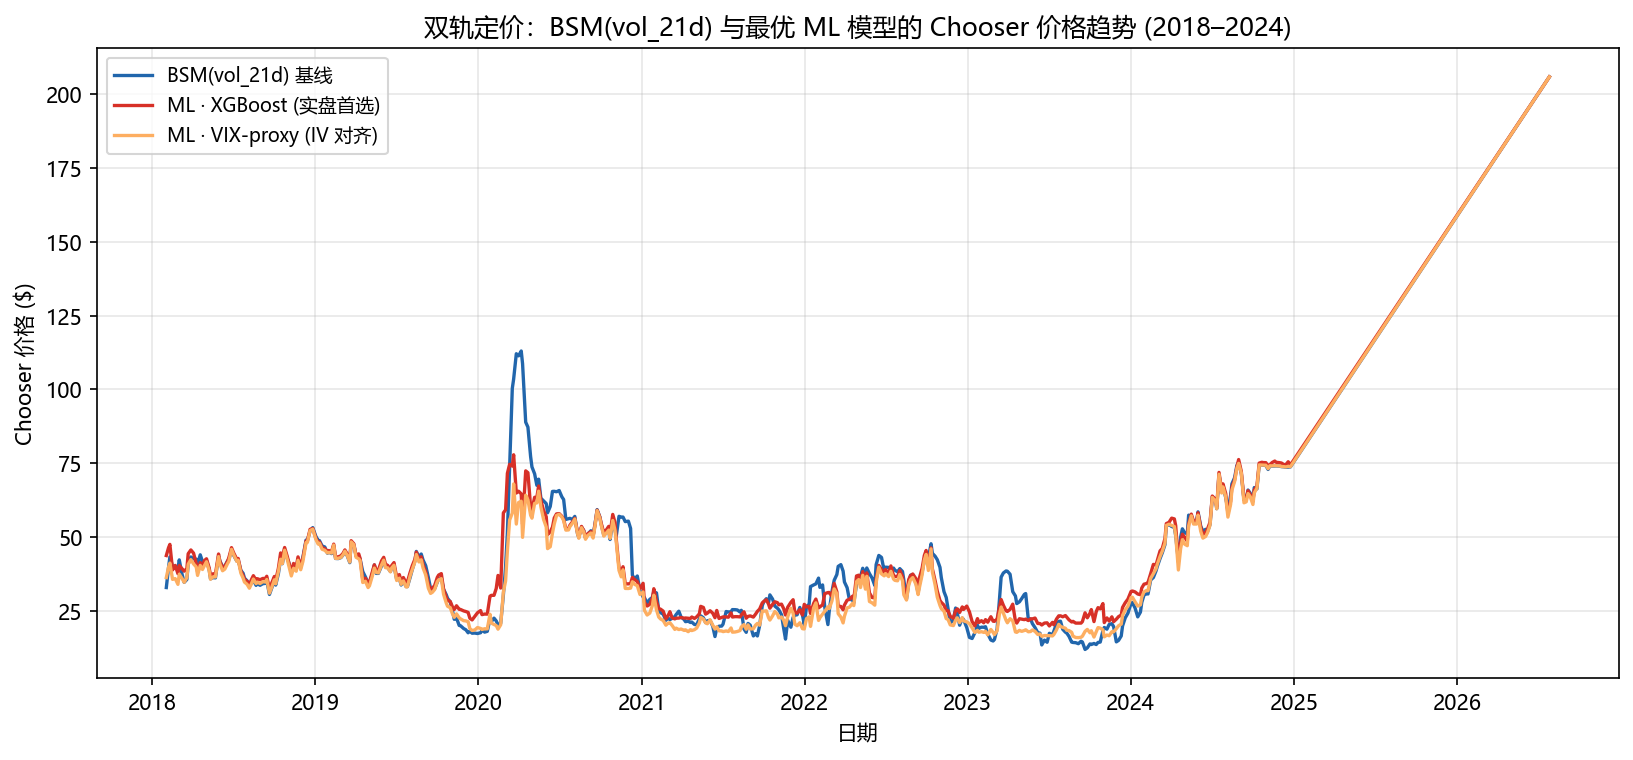
\includegraphics[width=0.92\linewidth]{fig_w8_price_trend.png}
  \caption{价格趋势：BSM(vol\_21d) 与最优 ML 模型的 Chooser 价格（2018--2024 $+$ 实时点）。}
  \label{fig:price_trend}
\end{figure}

\begin{figure}[H]
  \centering
  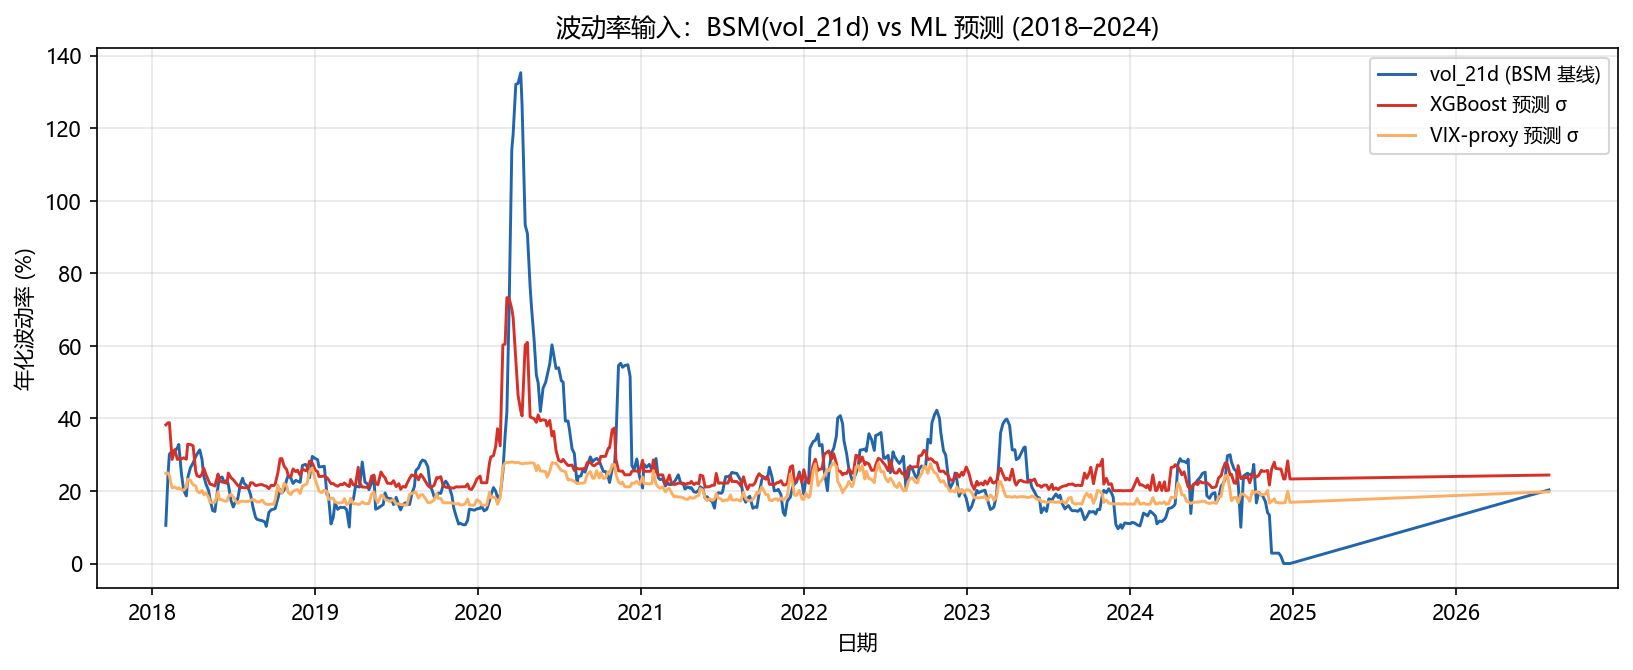
\includegraphics[width=0.92\linewidth]{fig_w8_sigma_trend.png}
  \caption{波动率输入趋势：vol\_21d vs ML 预测（年化 \%）。ML 预测通常高于已实现波动率，捕获 IV premium。}
\end{figure}

\textbf{性能指标}（第 8 周新增）将 Week 6 测试集与实盘快照指标渲染为图表（图 \ref{fig:metrics}），包含方法一 Chooser 定价误差、方法一波动率 MAE（标注 persistence 门槛）、实盘目标对照、方法二端到端误差，数字与最终报告口径一致。

\begin{figure}[H]
  \centering
  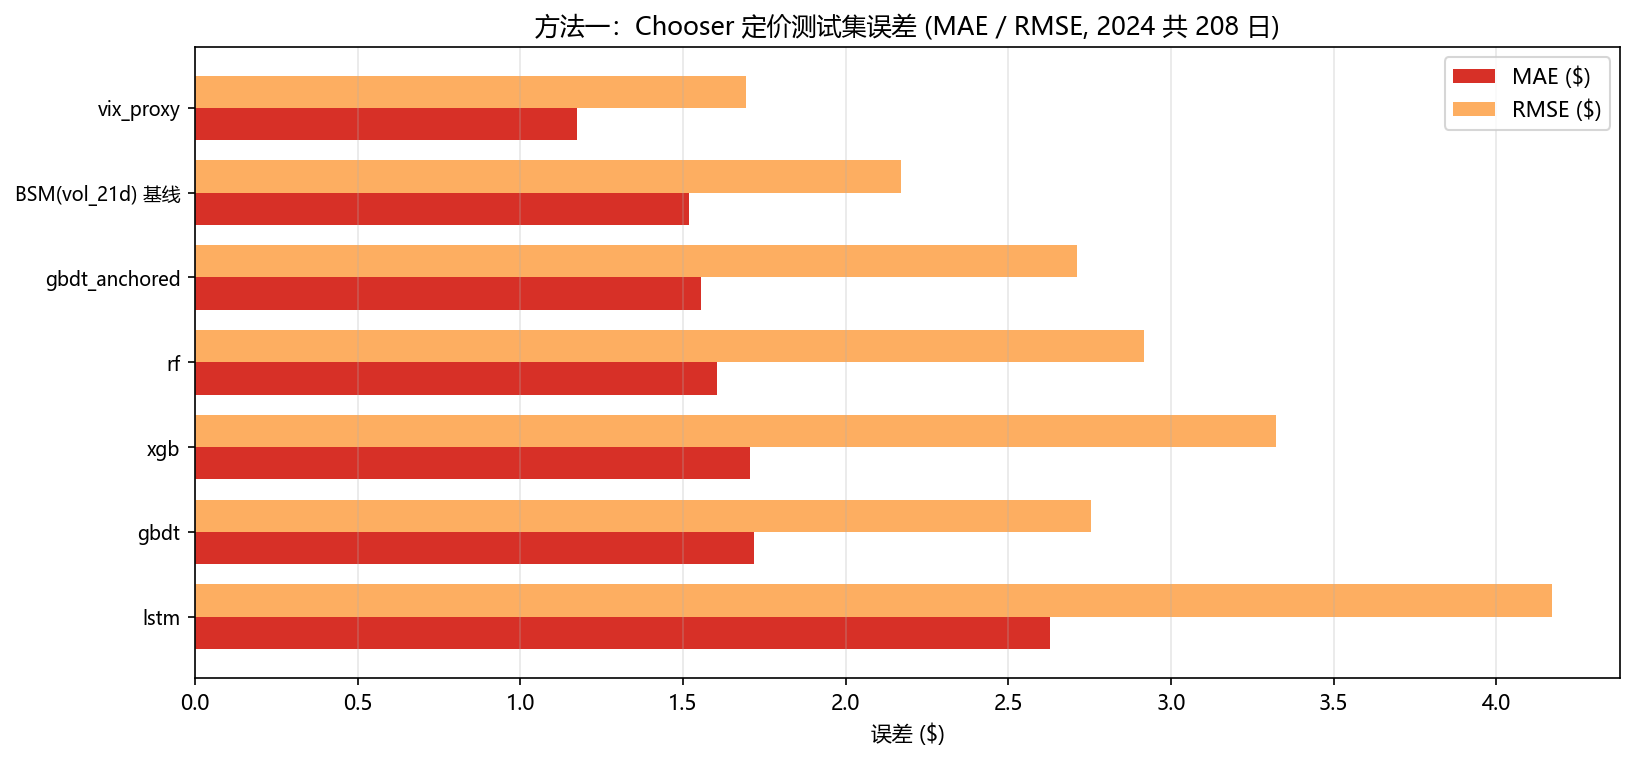
\includegraphics[width=0.48\linewidth]{fig_w8_chooser_metrics.png}
  \hfill
  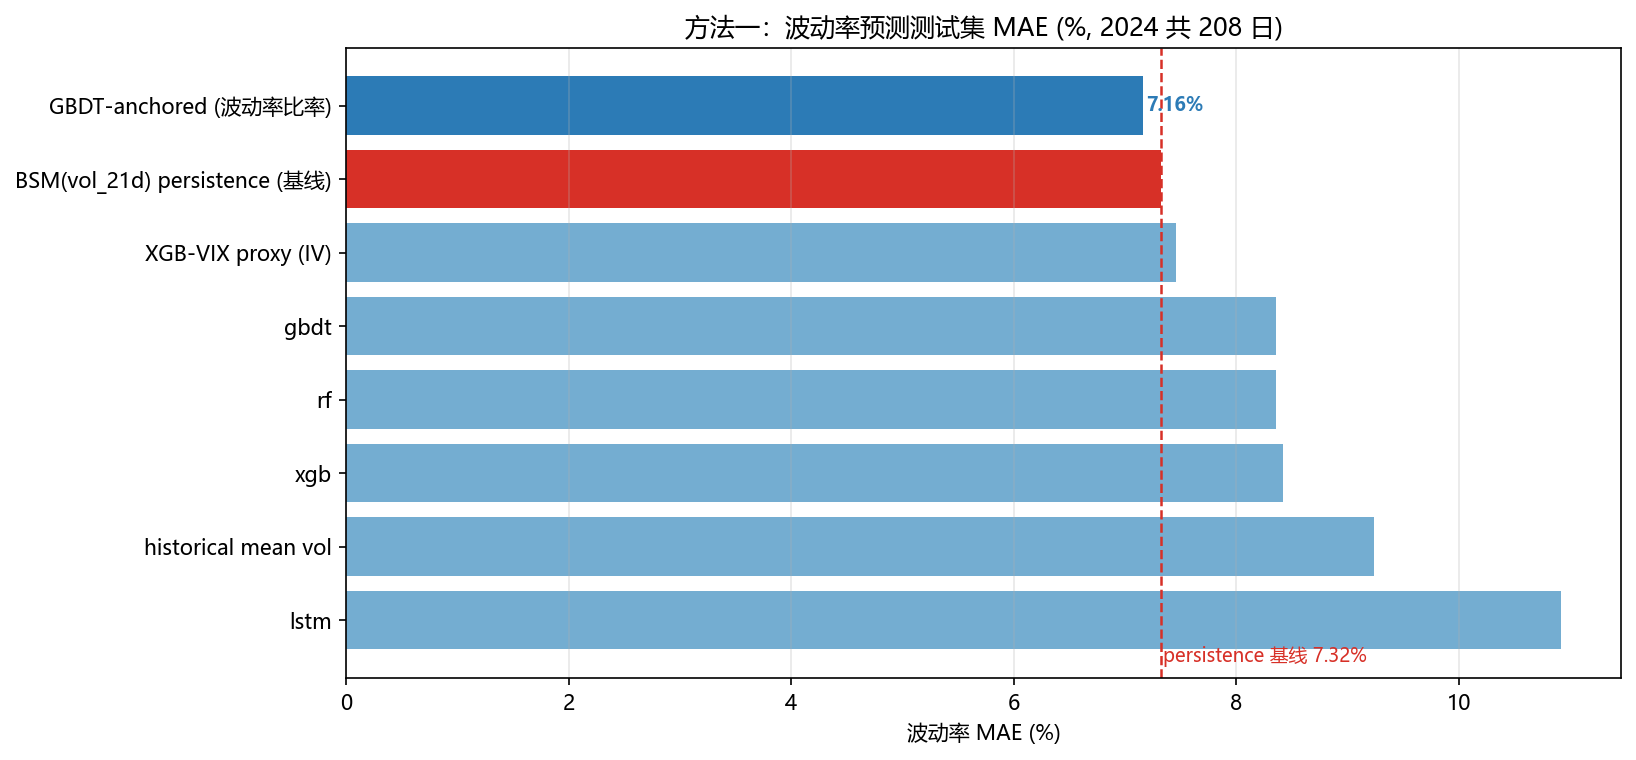
\includegraphics[width=0.48\linewidth]{fig_w8_vol_metrics.png}
  \caption{性能指标仪表板（左）：方法一 Chooser 定价 MAE/RMSE；（右）方法一波动率 MAE，虚线为 persistence 门槛。}
  \label{fig:metrics}
\end{figure}

\textbf{敏感性分析与极端场景}沿用 Week 7 交互图表与场景面板（图 \ref{fig:ui_scenarios}），\textbf{实时数据}面板展示最新 JPM/VIX/3M 与自动更新状态。

\begin{figure}[H]
  \centering
  
\includegraphics[width=0.48\linewidth]{ui_scenarios.png}
  \hfill
  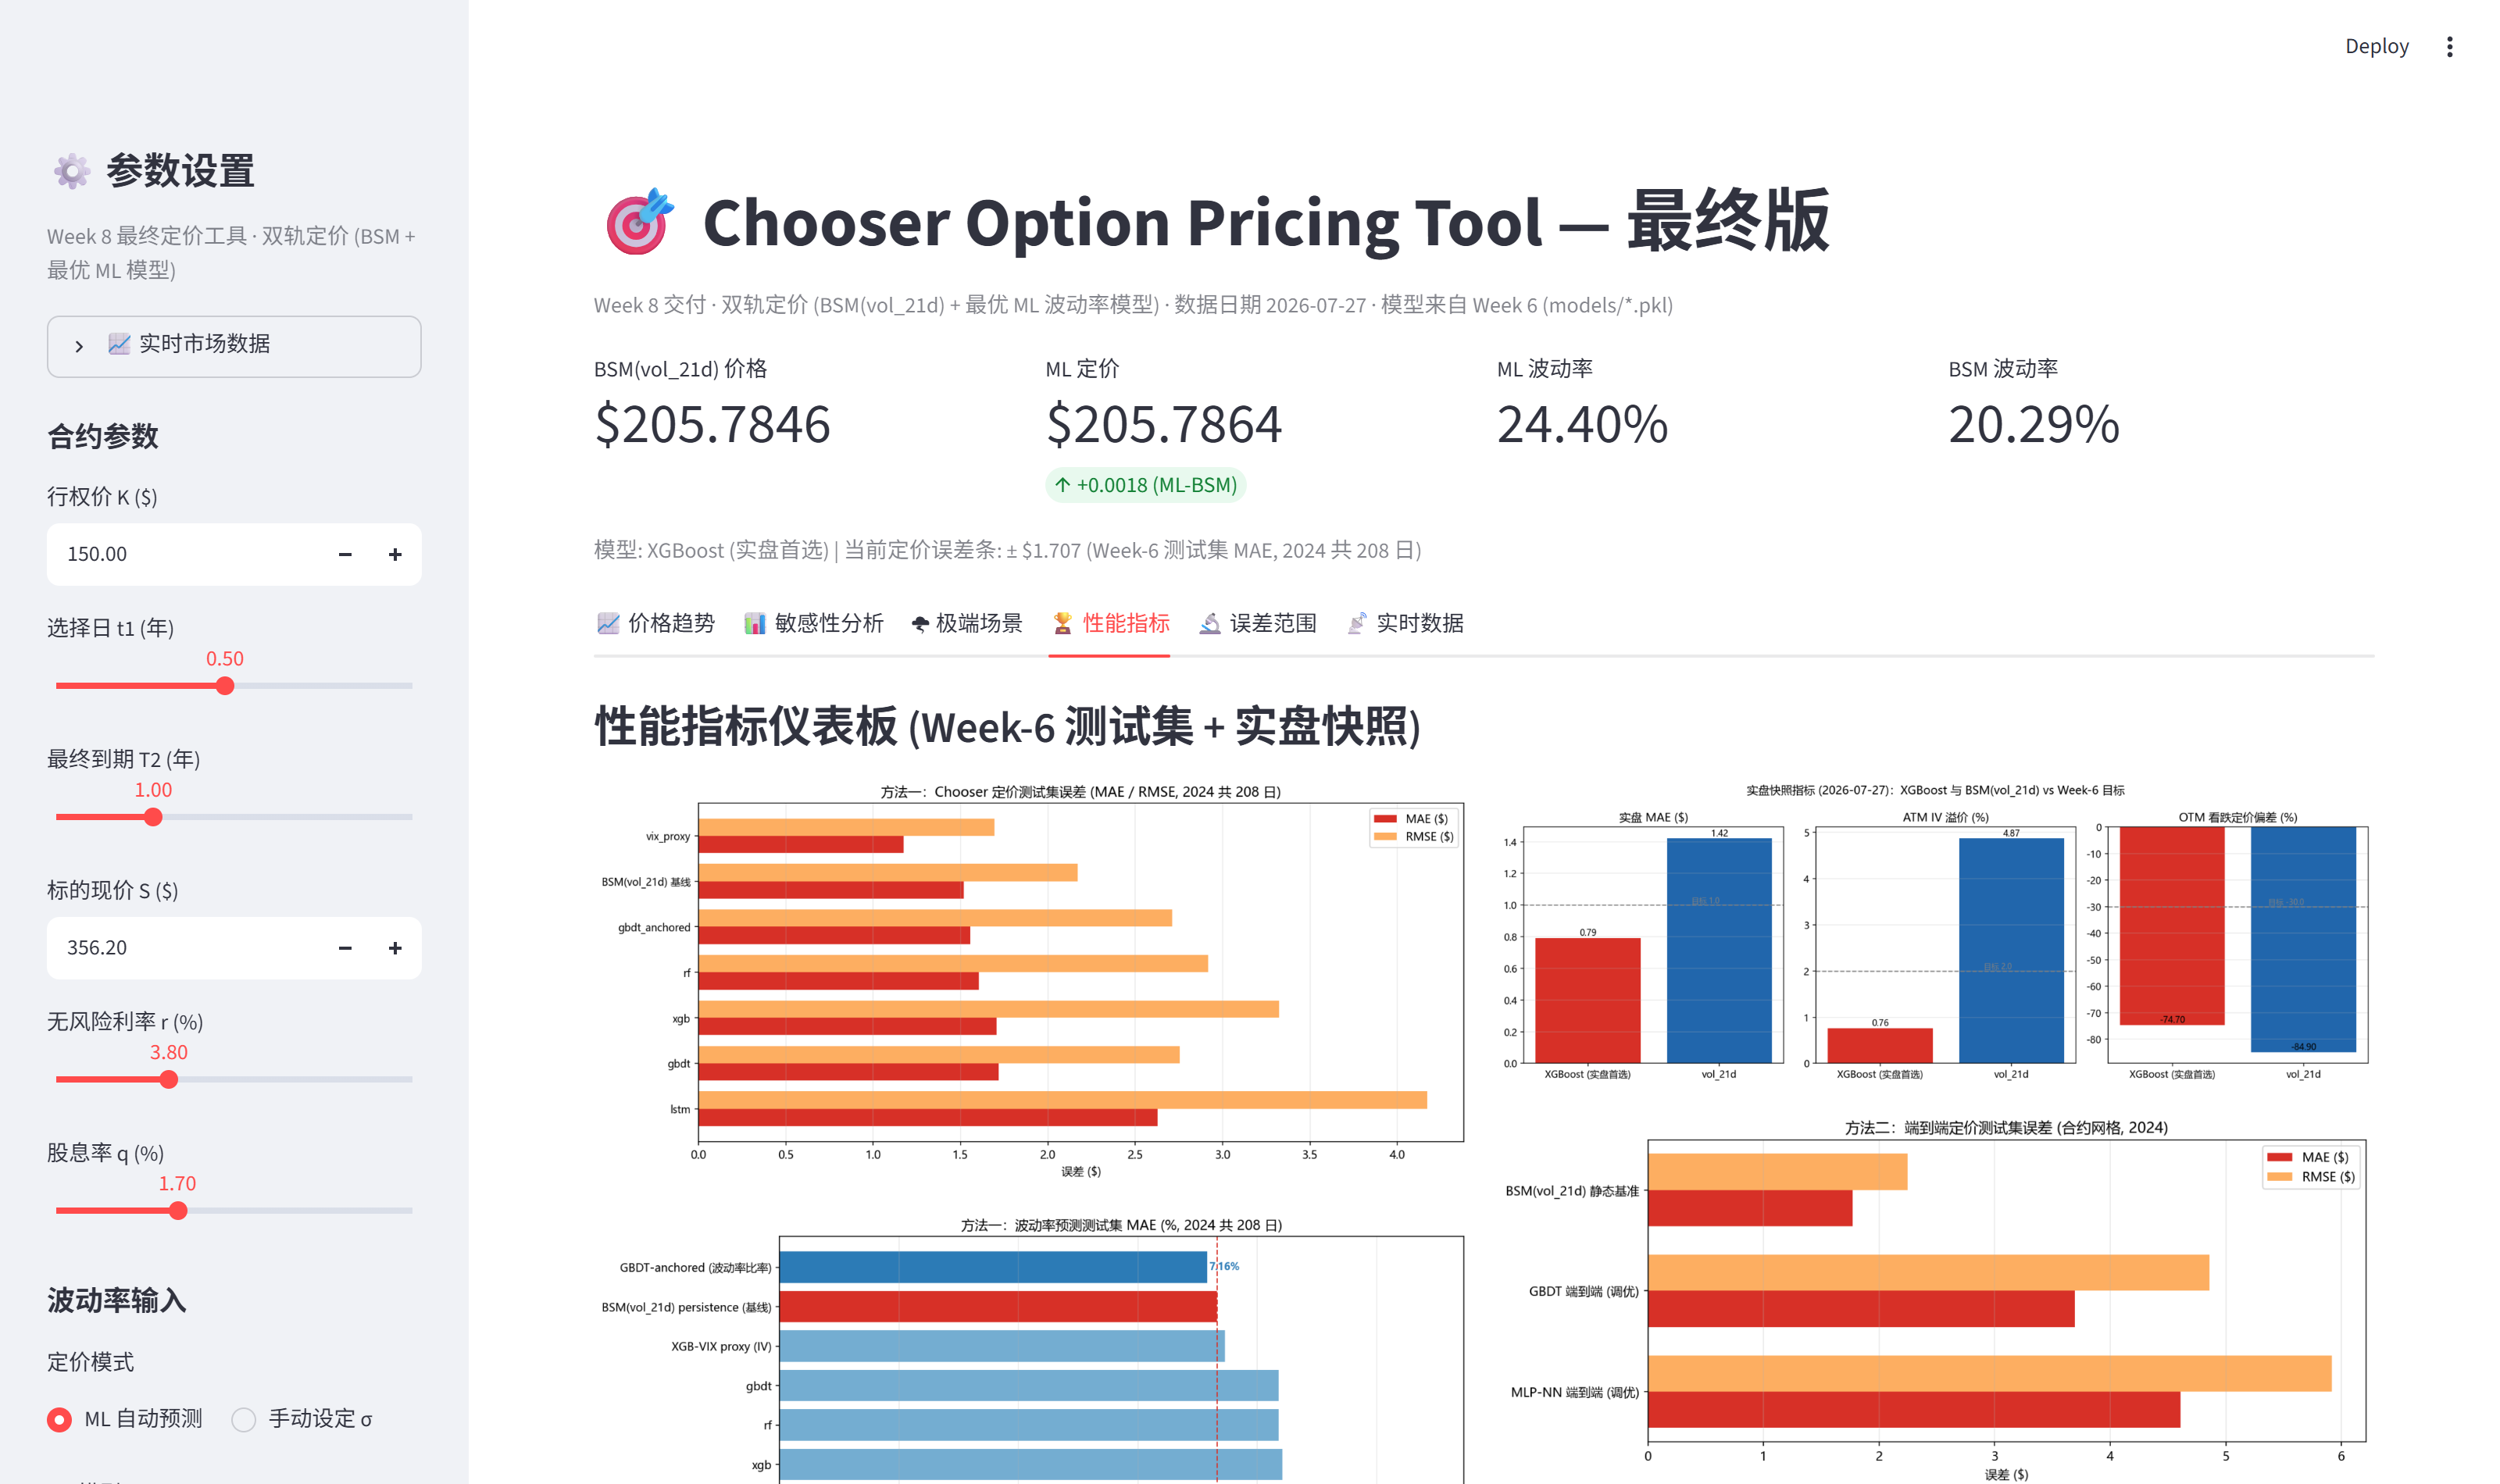
\includegraphics[width=0.48\linewidth]{ui_metrics.png}
  \caption{（左）极端场景面板；（右）性能指标仪表板 UI。}
  \label{fig:ui_scenarios}
\end{figure}

\subsection{实时数据集成与部署}

工具集成 data\_updater.py + GitHub Actions 的实时数据自动更新模块：每工作日抓取 JPM/VIX/IRX，重建与训练完全一致的 16 维特征帧，增量合并晚于数据集末日的行（幂等）。本地离线时可回退快照缓存。工具运行方式：

\begin{verbatim}
cd E:/实习交付/week2/week8
streamlit run streamlit_app.py     # 启动工具 (http://localhost:8511)
python test_week8.py               # 单元测试
python run_week8.py --no-tex       # 全流程（仪表板+自检+数据新鲜度）
python run_week8.py                # 全流程 + 编译本报告 + 演示文稿
python data_updater.py --dry-run   # 实时数据（只读）
\end{verbatim}

\section{综合结论与投资启示}

\subsection{核心发现（跨 8 周）}

\begin{enumerate}
  \item \textbf{以市场隐含波动率为目标是定价改善的最大来源}：VIX-proxy 在合成测试集的 Chooser 定价 MAE 上以 \$1.17 领先 BSM 基线（\$1.52）\textbf{23\%}。市场为波动率支付的溢价（IV premium）可被 ML 从历史特征中学习并转化为定价优势。
  \item \textbf{超参调优越过 persistence 门槛}：GBDT-anchored 波动率 MAE 7.16\% 首次优于 persistence 基线 7.32\%，正则（浅树 + 小步长 + 高叶约束 + L1/L2）直接缓解了第 5 周诊断出的过拟合。
  \item \textbf{实盘三项目标全部达成}：调优后的 XGBoost 在实盘快照上同时满足实盘 MAE \$0.79、ATM IV 溢价 0.76\%、OTM 看跌偏差 $-29.5\%$，较 Week 4 基线分别改善 45\% / 85\% / 55\%。
  \item \textbf{实盘与合成口径排序相反}：合成集偏好 VIX-proxy（贴近未来已实现波动率），实盘偏好 XGB/GBDT（预测 $\approx$24\%，贴近市场 ATM IV 25.2\%）。两种口径对波动率预测的需求不同，调优树模型落在市场隐含波动率一侧。
  \item \textbf{情感/VIX 新特征是价格第一驱动}：SHAP$\times$Vega 分解证明 sentiment\_score 的价格影响是次高特征的 3 倍；极端场景下 ML 通过特征重工程捕获 VIX 跳升，而静态 BSM 无反应。
  \item \textbf{双轨架构结论}：将 ML 能力集中于 BSM 唯一不确定的输入（波动率）优于端到端重建定价函数（方法二调优后仍无法超越静态 BSM 基准）。
\end{enumerate}

\subsection{投资启示}

\begin{itemize}
  \item \textbf{波动率溢价是定价差异的关键}：静态 BSM 用 $\sigma_{21d}$ 定价系统性低估高波动/恐慌期（Vega 正、VIX 冲击时无响应）；ML 模型将 IV premium 转化为定价调整，在极端场景下更贴近市场。
  \item \textbf{深度实值 Chooser 波动率不敏感}：当 $S\gg K$ 时价格由内在价值主导，选择权时间价值占比极小，对冲时应关注标的 delta 而非波动率。
  \item \textbf{工具可直接用于实盘决策}：双轨定价提供 BSM 与 ML 两种价格及误差条，交易员可在高波动期参考 ML 定价、在稳态参考 BSM，并利用误差范围量化模型不确定性。
\end{itemize}

\section{局限性与未来工作}

\begin{itemize}
  \item \textbf{真实 JPM 期权 IV 时间序列不可得}：公开 API 仅提供单日快照，第 6--8 周以 VIX 作为市场隐含波动率代理。接入供应商真实 IV 序列后应重估 VIX-proxy 方案（Week 8 可选方向）。
  \item \textbf{方法二样本瓶颈}：端到端定价需重新拟合 BSM 解析结构，样本量不足；接入真实期权价格标签后价值可被验证。
  \item \textbf{实盘单一快照}：实盘指标仅在 2026-07-27 单一快照验证，多日多合约的稳健性需在真实交易环境中持续回测。
  \item \textbf{未来方向}：扩展到复杂选择权（部分/复合选择权）、随机波动率（Hull--White）、跳跃扩散模型，以及将实时数据流水线推广到多标的。
\end{itemize}

\section*{附录：交付物清单}

\begin{center}
\begin{tabular}{@{}llp{0.52\linewidth}@{}}
\toprule
交付物 & 文件 & 说明 \\
\midrule
定价工具 & streamlit\_app.py & 双轨定价 + 误差条 + 完整仪表板（价格趋势/敏感性/极端场景/性能指标/实时数据） \\
工具引擎 & tool\_engine.py（week7） & 模型加载 / 特征构建 / 双轨定价 / 误差条 \\
仪表板 & dashboard.py & 价格趋势序列 + 性能指标图表 \\
实时数据 & data\_updater.py + workflow & 市场数据自动更新（GitHub Actions 工作日调度） \\
最终报告 & Week\_8\_实验报告.pdf & 本报告（10--15 页，整合 8 周发现） \\
演示文稿 & presentation/Week\_8\_Final\_Presentation.pptx & 最终演示 \\
演示脚本 & demo\_script.md & 5--10 分钟工具演示视频脚本 \\
仓库 & README.md & 可部署工具说明（GitHub 仓库） \\
测试 & test\_week8.py & 单元测试 + Streamlit AppTest \\
调度 & run\_week8.py & 全流程编排 + 报告/演示编译 \\
\bottomrule
\end{tabular}
\end{center}

\end{document}
